\documentclass{article}
\usepackage[T1]{fontenc}
\usepackage{lmodern}
\usepackage{graphicx}
\usepackage{amsmath,amssymb}
\usepackage[a4paper,margin=2cm]{geometry}
\usepackage[absolute,overlay]{textpos}
\setlength{\TPHorizModule}{1mm}
\setlength{\TPVertModule}{1mm}
\usepackage[indonesian]{babel}
\usepackage{hyperref}
\setlength{\emergencystretch}{2em}
% unit: Halaman 13

\begin{document}

% === Halaman 13 (llm) ===

\begin{itemize}
  \item \textbf{Penggunaan \textit{tablet wax}}

  Orang-orang Yunani kuno menulis pesan rahasia di atas kayu yang kemudian ditutup dengan lilin (\textit{wax}).
\end{itemize}

\vspace{10mm}

Di dalam bukunya, Heradatus menceritakan Demaratus mengirim peringatan tentang serangan yang akan datang ke Yunani dengan menulis langsung pada tablet kayu yang kemudian dilapisi lilin dari lebah.

% deskripsi: Ilustrasi tablet lilin (wax tablet) kuno yang terdiri dari dua papan kayu dengan lapisan lilin gelap di dalamnya dan alat tulis kayu (stylus).
% bbox normalisasi: [0.2930, 0.5550, 0.6750, 0.9050]
\begin{textblock*}{80.22mm}(61.53mm,164.84mm)
\noindent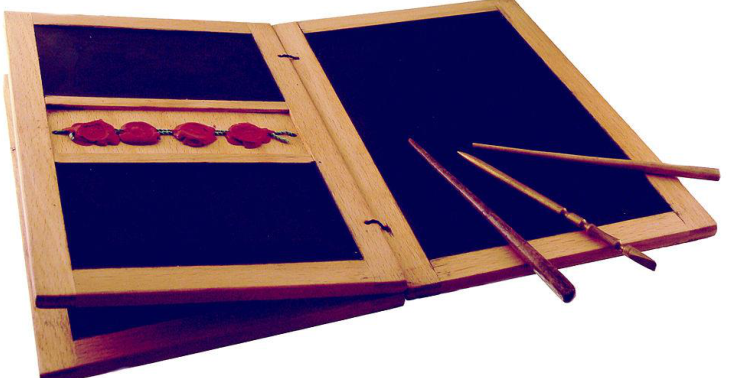
\includegraphics[width=80.22mm,height=103.95mm]{../../images/llm/page_013_img_01.png}%
\end{textblock*}

\end{document}
